\documentclass[twoside]{book}
\newif\ifpdf
\ifx\pdfoutput\undefined
\pdffalse % we are not running PDFLaTeX
\else
\pdfoutput=1 % we are running PDFLaTeX
\pdftrue
\fi
%\usepackage{times}
%\usepackage{amsmath}
\usepackage{calc}
\usepackage[latin1]{inputenc}
\usepackage{FFF}
\usepackage{amsfonts}
\usepackage{amsmath}
\usepackage{hyperref}
\usepackage{FFF}
\usepackage{makeidx}
\usepackage{color}
\usepackage{multicol}
\usepackage{graphicx}
%\usepackage{dessin}
\topmargin -1.54cm
\oddsidemargin 0cm   %marge a 2 cm
\evensidemargin 0cm  %marge a 2 cm
\newcommand{\indente}{\hbox to \parindent {\hss}}
\parindent 0cm
\headsep 0.5cm
\topskip .5cm
\footskip 1cm
\headheight 1.0cm
\textwidth  16.5cm
%  \parindent 0cm
\textheight 24cm
\def\freefempp{\texttt{freefem++ }}
\def\textRed{\color{red}}
\def\textBlack{\color{black}}
\def\Blue#1{\textcolor{blue}{#1}}
\def\Black#1{\textcolor{black}{#1}}
\def\Red#1{\textcolor{red}{#1}}
\def\Magenta#1{\textcolor{magenta}{#1}}
\def\hin{\hbox{ in }}
\def\hon{\hbox{ on }}
\def\Cpp{\texttt{C++~}}
\def\R{\mathrm{I\!R}}
\def\example{\textbf{Example:}}
\def\eq#1{\Blue{\[#1\]}}
\def\R{\mathbb{R}}
\def\Z{\mathbb{Z}}
\def\itemtt[#1]{ \item[\texttt{#1}]}
\def\plot[#1]#2#3{\begin{figure}[hbt]
\begin{center}
    \includegraphics*[#1]{#2}
\end{center}
\caption{\label{#2} #3}
\end{figure}
}
\def\Ostream{\texttt{ostream}}
\def\Istream{\texttt{istream}}
\def\Bool{\texttt{bool}}
\def\Real{\texttt{real}}
\def\Int{\texttt{int}}
\def\vecttwo#1#2{\left|\begin{smallmatrix} #1 \\ #2 \end{smallmatrix}\right.}
\def\vdeux(#1,#2){\left|\begin{smallmatrix} #1 \\ #2 \end{smallmatrix}\right.}
\def\HLINE#1{\hbox to \hsize {#1}}
\def\twoplot[#1]#2#3#4#5{
\begin{figure}[hbt]
\begin{multicols}{2}
\begin{center}
    \includegraphics*[#1]{#2}
    \caption{\label{#2} #4}
\end{center}
\begin{center}
    \includegraphics*[#1]{#3}
    \caption{\label{#3} #5}
\end{center}
\end{multicols}
\end{figure}
}% end twoplot macro
\newtheorem{remark}{\textbf{Remark}}
\newtheorem{bug}{\textbf{Bug:}}
\newtheorem{proposition}{\textbf{Proposition}}
\newtheorem{algorithm}{\textbf{Algorithm}}
\newenvironment{ttlist}
   {\begin{list}{}{\renewcommand{\makelabel}[1]{\texttt{##1}\hfil}%
        \setlength{\labelwidth}{3cm}
        \setlength{\leftmargin}{\labelwidth+\labelsep}
    }}%
   {\end{list}}


\begin{document}
\graphicspath{{./}{plots/}}
\ifpdf
\DeclareGraphicsExtensions{.pdf, .jpg, .tif}
\else
\DeclareGraphicsExtensions{.eps,.ps, .jpg}
\fi

\let\subsubsection\subsection
\let\subsection\section
\let\section\chapter



In this exemple,  we do metric mesh adaption and we computionj the classical 
residual error indicator $\eta_{K}$ on the element $K$ for the Poisson problem.

First, we solve the same problem as in a previous example.
\bFF

border ba(t=0,1.0){x=t;   y=0;  label=1;}; // comment 
border bb(t=0,0.5){x=1;   y=t;  label=2;};
border bc(t=0,0.5){x=1-t; y=0.5;label=3;};
border bd(t=0.5,1){x=0.5; y=t;  label=4;};
border be(t=0.5,1){x=1-t; y=1;  label=5;};
border bf(t=0.0,1){x=0;   y=1-t;label=6;};
mesh Th = buildmesh (ba(6) + bb(4) + bc(4) +bd(4) + be(4) + bf(6));
fespace Vh(Th,P2);
Vh u,v;
real error=0.01;
func f=(x-y);
problem Probem1(u,v,solver=CG,eps=1.0e-6) =   int2d(Th,qforder=5)( u*v*1.0e-10+  dx(u)*dx(v) + dy(u)*dy(v))  + int2d(Th,qforder=5)( -f*v);
\eFF

\index{jump}\index{intalledges}\index{square}\index{lenEdge}\index{hTriangle}%\index{area}
 \index{qforder=}
Now, the local  error indicator $\eta_{K}$ is:
\def\Th{\mathcal{T}_{h}}
\def\AK{\mathcal{E}_{K}}

  $$\eta_{K} =\left(  h_{K}^{2} || f -\Delta u_{{h}} ||_{L^{2}(K)}^{2} +\sum_{e\in \AK} h_{e} \,||\, [ \frac{\partial u_{h}}{\partial n_{k}}] \,||^{2}_{L^{2}(e)} \right)^{\frac{1}{2}}
   $$
   where $h_{K}$ is the longest's edge of  $K$, $\AK$ is the set of $K$ edge not on 
      $\Gamma=\partial \Omega$, $n_{K}$ is the  outside unit normal to $K$, $h_{e}$ is the length of edge $e$,
   $[ g ]$ is the jump of the function $g$ across edge (left value minus rigth value). 
 
 
Of coarse, we can use a variational form to compute $\eta_{K}^{2}$,
with test function constante function by triangle.
\bFF
  
fespace Nh(Th,P0); // the set function constante function by triangle Nh eta,logeta;
varf indicator2(uu,chiK) = 
       intalledges(Th)(chiK*lenEdge*square(jump(N.x*dx(u)+N.y*dy(u))))     +int2d(Th)(chiK*square(hTriangle*(f-dxx(u)-dyy(u))) );
\eFF

\bFF

for (int i=0;i< 4;i++)
{   Probem1;
  cout << u[].min << " " << u[].max << endl; 
  plot(u,wait=1);
   cout << " indicator2 " << endl; 
  eta[] = indicator2(0,Nh);
  eta=sqrt(eta);
  cout << eta[].min << " " << eta[].max << endl;
  plot(eta,fill=1,wait=1,cmm="indicator density ",ps="rhoP2.eps");
  Th=adaptmesh(Th,[dx(u),dy(u)],err=error,anisomax=1);
  plot(Th,wait=1);
  u=u;
  eta=eta;
  error = error/2;
} ;
\eFF

If the method is correct, we espect an almost constant function $\eta$, as you can see 
on the graphics .label{fig rhop2}.
\begin{figure}[hbt]
\begin{center}
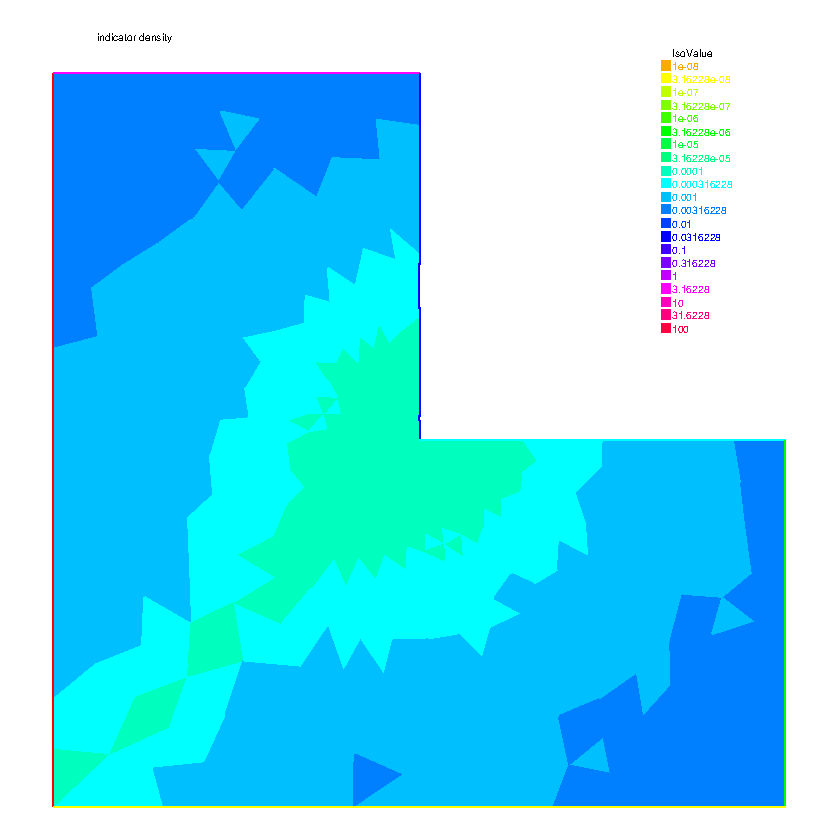
\includegraphics[height=8cm]{rhoP2.ps} 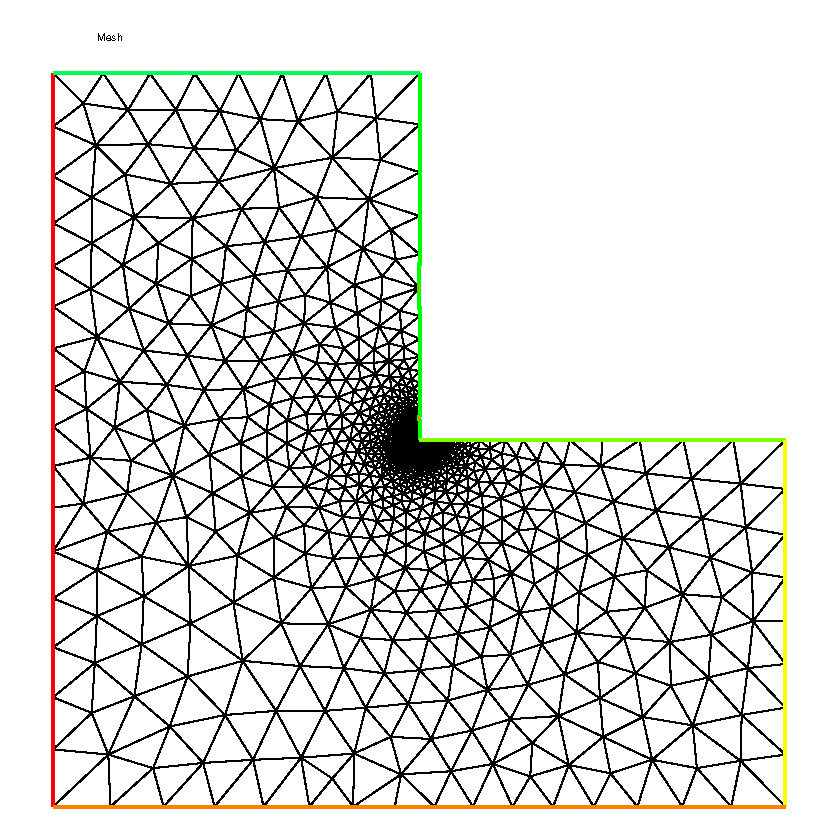
\includegraphics[height=8cm]{ThrhoP2.eps}
\end{center}
\caption{Density of the error indicator  with isotropic $P^{2}$ metric }
\end{figure}


\end{document}